\documentclass{jsarticle}

\usepackage[dvipdfmx]{graphicx}
\usepackage{
    amsmath,
    amsfonts,
    bm
}

\def\q{\bm{q}}
\def\k{\bm{k}}

\title{
    Transformerモデルのコンテキスト拡張手法
}
\author{平田 蓮}
\date{2024年7月10日}

\begin{document}
\maketitle

まずはじめに、LLaMAなどで用いられている主流な位置エンコーディング手法であるRoPEの説明を行う。
その後、シーケンス拡張を行う為に提案された手法を取り上げる。

\section{RoPE}
    Jianlinら\cite{rope}によって提唱された、
    位置エンコーディングを加算ではなく乗算で行うアプローチ。
    LLaMAなどで用いられており、現在主流である。
    QueryとKeyに回転行列をかけて、ベクトルを回転させることで位置情報を乗せる。
    トークンの位置ごとに徐々に回転角を増していくため、
    相対位置情報も反映されていると考えられている。

    回転行列は、次の式で与えられる。
    \begin{align}
        R &= \begin{pmatrix}
                \cos m\theta_1 & -\sin m\theta_1 & 0 & 0 & \cdots & 0 & 0 \\
                \sin m\theta_1 & \cos m\theta_1 & 0 & 0 & \cdots & 0 & 0 \\
                0 & 0 & \cos m\theta_2 & -\sin m\theta_2 & \cdots & 0 & 0 \\
                0 & 0 & \sin m\theta_2 & \cos m\theta_2 & \cdots & 0 & 0 \\
                \vdots & \vdots & \vdots & \vdots & \ddots & \vdots & \vdots \\
                0 & 0 & 0 & 0 & \cdots & \cos m\theta_\frac{D}{2} & -\sin m\theta_\frac{D}{2} \\
                0 & 0 & 0 & 0 & \cdots & \sin m\theta_\frac{D}{2} & \cos m\theta_\frac{D}{2}
            \end{pmatrix} \label{equ:rope} \\
        \theta_i &= 10000^{-\frac{2(i-1)}{D}} \ \left(i = 1, 2, \cdots, \frac{D}{2}\right) \nonumber
    \end{align}
    ここで、$m$はトークン位置、$D$は埋め込みの次元である。
    つまり、トークン位置が後ろに行くほど、回転角が大きくなる。
    この回転行列はベクトルの$D$次元空間を2次元ずつ取って、
    その2軸が成す平面において回転させる。
    これを用いて計算した$Q' = R {}^t\!Q, K' = R {}^t\!K$により
    Attention行列を計算する。
    \begin{figure}[ht]
        \centering
        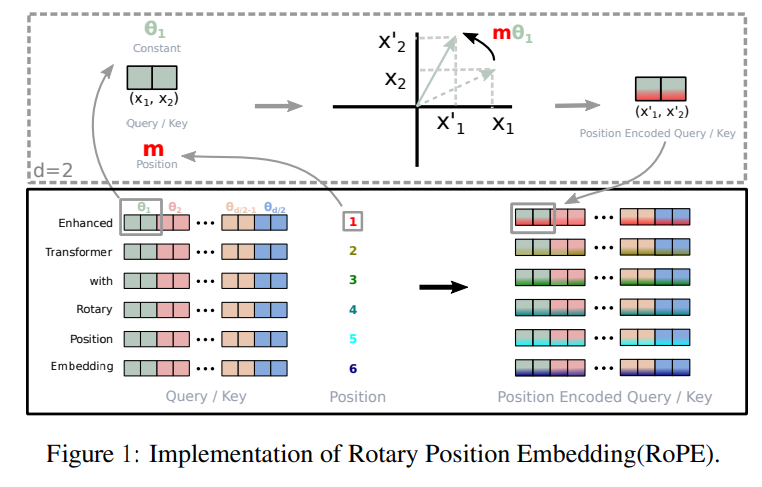
\includegraphics[width=.8\hsize]{rope_image.png}
        \caption{RoPE\cite{rope}}
    \end{figure}

\section{シーケンスの拡張}
    \subsection{Position Interpolation}
        RoPEのシンプルな拡張として、
        Shouyuanら\cite{inter}とkaiokendev\cite{kaiokendev}
        によって提案されたPosition Interpolationが挙げられる。
        これは、RoPEのトークン位置を元のコンテキスト長と新しいコンテキスト長の比率を
        用いてスケールするものである。
        すなわち、式\ref{equ:rope}において、
        $m\rightarrow \frac{L}{L'}m$とする。
        ここで、$L$は元のコンテキスト長、$L'$は拡張したコンテキスト長である。
        今後、$\frac{L'}{L}$をスケール倍率と呼ぶ。
        
        この手法は、拡張したコンテキスト長で少数ショット学習を行うことで
        モデルの性能を落とさずにコンテキストを拡張できることが示された\cite{inter}。
        しかし、一定より高いスケール倍率を用いると、
        性能が低下することも確認されている。

    \subsection{YaRN}
        RoPEにおける$d$次元目の回転角を$\theta_d$としたとき、
        RoPEにおける波長$\lambda_d=\frac{2\pi}{\theta_d}$を定義する。
        波長は、その次元に対する位置エンコーディングの回転が一周するのに必要なトークン数を表す。
        Bowenら\cite{yarn}は、この波長に着目し、
        RoPEのコンテキスト拡張を行った。

        埋め込みの後ろの方の次元の一部の範囲において、
        学習したコンテキスト長よりも波長が長い次元が存在する。
        つまり、その次元においては位置エンコーディングが回転領域で均等に分布していない。
        このような場合は、Position Interpolationを行っても、
        位置エンコーディングの絶対位置の情報がそのまま残ってしまうことが危惧される。
        逆に、波長が短い次元においては、
        絶対位置の情報が消えてしまい、相対位置の情報しか残っていないと考えられる。

        加えて、先述の通りPosition Interpolationを高いスケール倍率で行うと性能が低下するが、
        これはスケール倍率を高くすればするほど距離が近いトークン同士の
        位置エンコーディングの差異が小さくなり、
        関係性をうまくモデルが認識できなくなっていることが原因であると考えられる。

        以上の仮定をもとに、Position Interpolationに次のような変更を行った。
        \begin{itemize}
            \item $\lambda_d$が$L$に対して十分に小さい次元ではスケーリングを行わない
            \item $\lambda_d$が$L$以上の次元では、$L'=\lambda_d$としたスケーリングを行う
            \item 上二つの間の次元領域では、波長の長さに応じて回転角を調整する
        \end{itemize}
        これは、二つのハイパーパラメータ$\alpha,\beta$を用いて以下の式で表される。
        \begin{align*}
            \gamma(r) &= \left\{ \begin{aligned}
                &0 \ &(r < \alpha) \\
                &1 \ &(r > \beta) \\
                &\frac{r-\alpha}{\beta-\alpha} \ &(\mathrm{otherwise})
            \end{aligned}\right. \\
            h(\theta_d) &= \left(1-\gamma\left(\frac{L}{\lambda_d}\right)\right)\frac{L}{L'}\theta_d + \gamma\left(\frac{L}{\lambda_d}\right)\theta_d
        \end{align*}
        $r$は波長に対する元のコンテキスト長の比であり、
        $\gamma$はこの比をもとに元の回転角とスケールした回転角それぞれを用いる
        比率を計算する。
        YaRNではPosition Interpolationと違い、
        $m$ではなく$\theta_d'=h(\theta_d)$として回転角に対してスケーリングを行うことに注意されたい。

        \subsubsection{実験結果}
            二つの実験を通してYaRNの性能が評価された。
            評価はPerplexityの比較で行われた。
            各モデルのPerplexityを表\ref{tab:yarn}に示す。
            表中にあるPIはPosition Interpolationを示し、
            NTKは、bloc97\cite{ntk}によって提案された別のRoPEの拡張手法である。

            \begin{figure}[ht]
                \caption{YaRNの性能評価\cite{yarn}。$s$はスケーリング倍率}
                \label{tab:yarn}
                \begin{center}
                    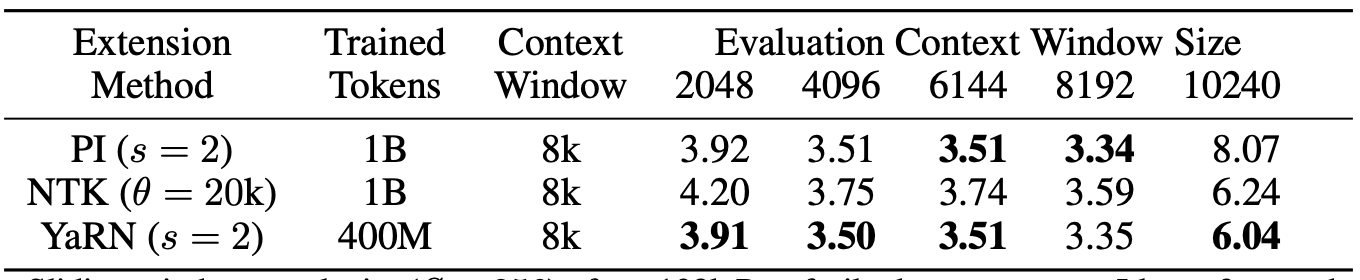
\includegraphics[width=.8\hsize]{yarn1.png}
                    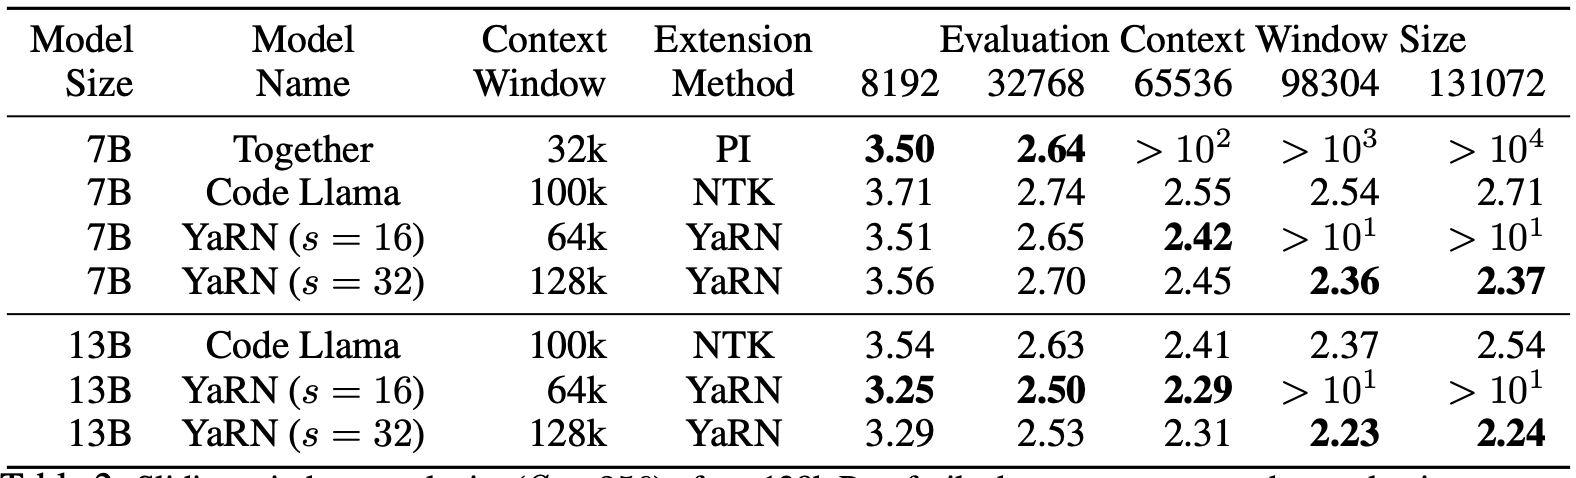
\includegraphics[width=\hsize]{yarn2.png}
                \end{center}
            \end{figure}

            上の表では、各手法に対してYaRNが少ない学習量でも優位であることが示された。
            下の表では、YaRNが高いスケーリング倍率でも有効であることが示された。

    \subsection{LongNet}
        LongNetは、Jiayuら\cite{longnet}によって提案されたモデルで、
        後述するDialated Attentionという構造を用いて
        コンテキスト長を10億まで拡張できることを示した。

        \subsubsection{Dialated Attention}
            Dialated Attentionは、
            トークンのAttentionを計算する際に、
            入力を複数の大きさのブロックに分割する。
            ブロックの大きさに応じて、
            Attentionを計算するトークンの間隔を広げ、
            一定の大きさの入力としている。
            これらの結果を合算し、離れた位置にあるトークン同士の依存関係も捉えている。
            Dialated Attentionの概念図を図\ref{fig:dialated}に示す。
            \begin{figure}[ht]
                \centering
                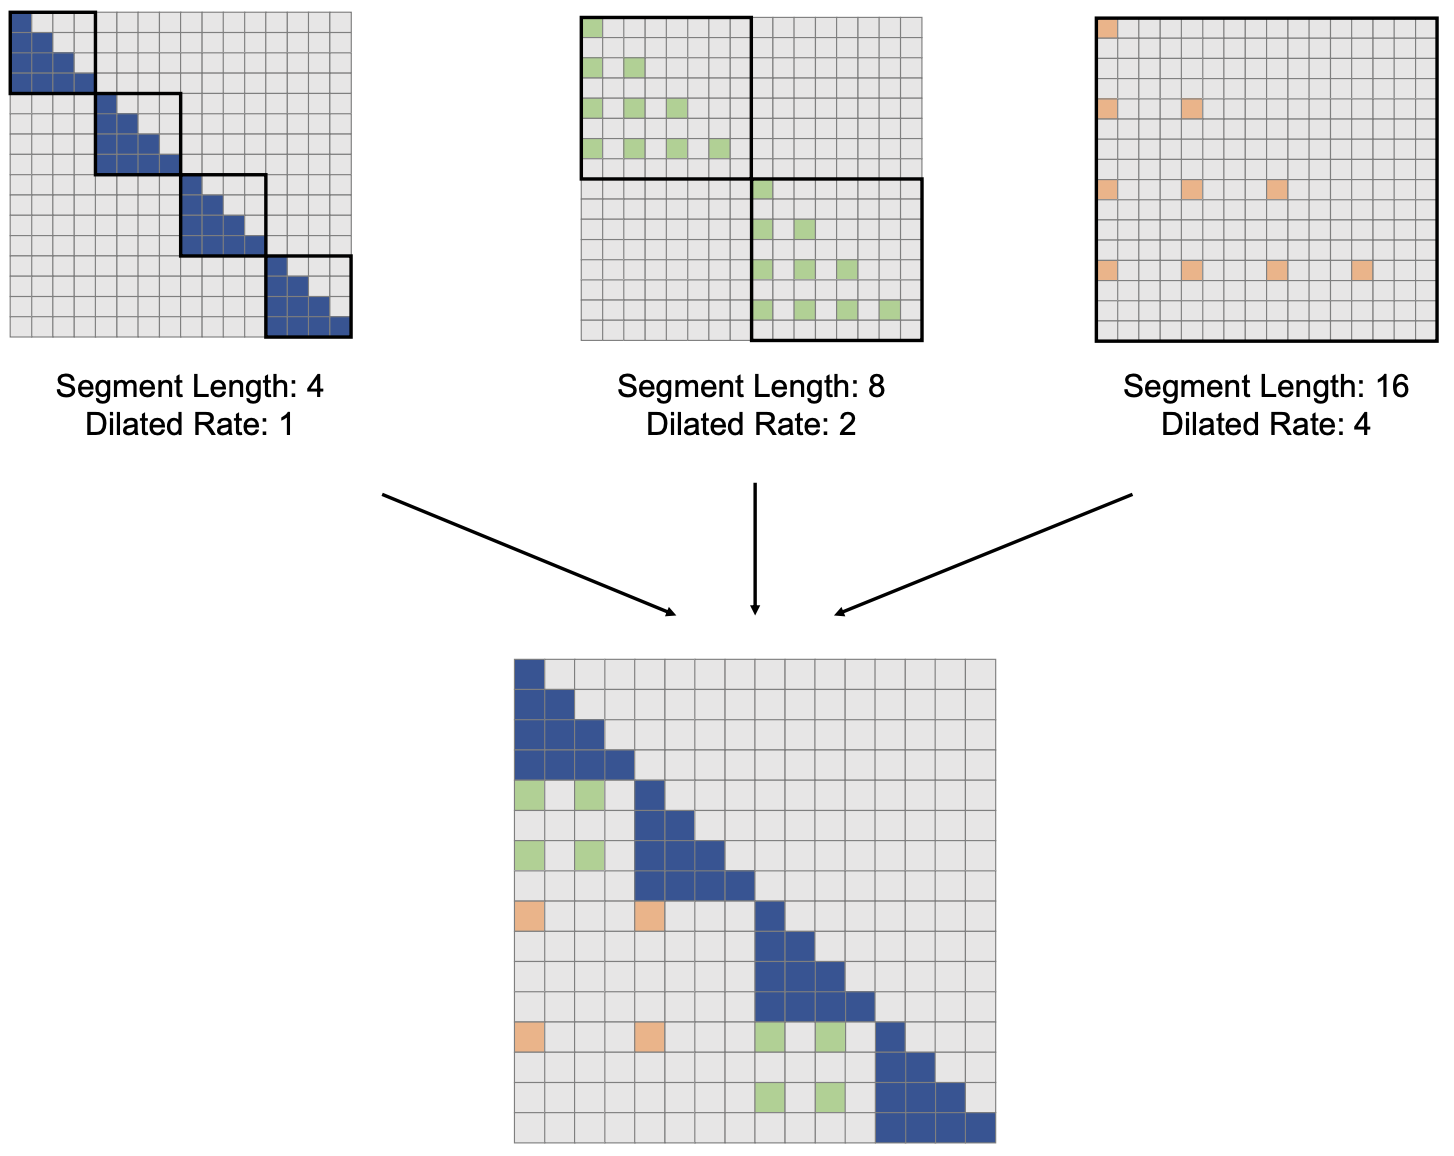
\includegraphics[width=\hsize]{dialated.png}
                \caption{Dialated Attention\cite{longnet}}
                \label{fig:dialated}
            \end{figure}
            
            さらに、各Attention headにおいてAttentionを計算するトークンのパターンを変更する。
            これにより、すべてのトークン間の依存関係を捉えられる。
            \begin{figure}[ht]
                \centering
                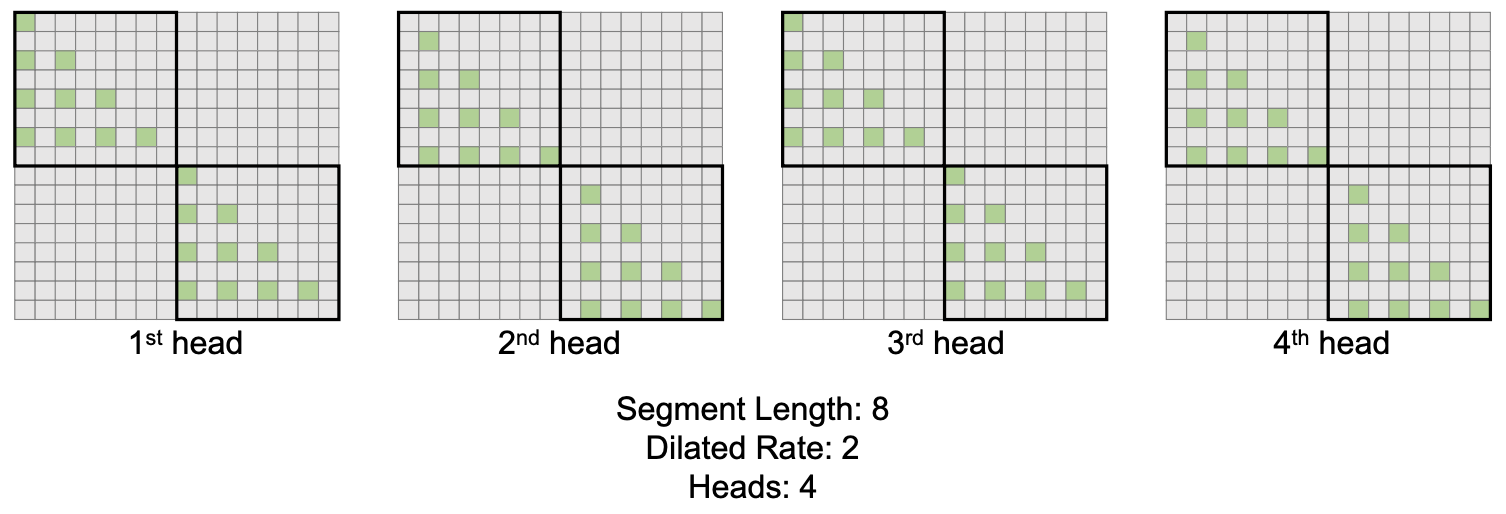
\includegraphics[width=\hsize]{dialated_pattern.png}
                \caption{Attention headごとのパターン\cite{longnet}}
            \end{figure}

        \subsubsection{実験結果}
            LongNetでは、Dialated Attentionに加え、
            時間計算量を抑える為に、
            分散アルゴリズムを用いてトークン長と埋め込み次元に対する線形時間で学習が行われた。
            32kまでのコンテキスト長でベースのTransformerモデルと同様の性能を発揮するこが確認され、
            さらにコンテキスト長を拡張しても性能が低下しないことが確認された。
            これにより、コンテキスト長を10億まで拡張できると結論づけられた。
            ベースモデルとのPerplexityの比較を表\ref{tab:longnet}に示す。
            \begin{figure}[ht]
                \caption{LongNetの性能\cite{longnet}}
                \label{tab:longnet}
                \centering
                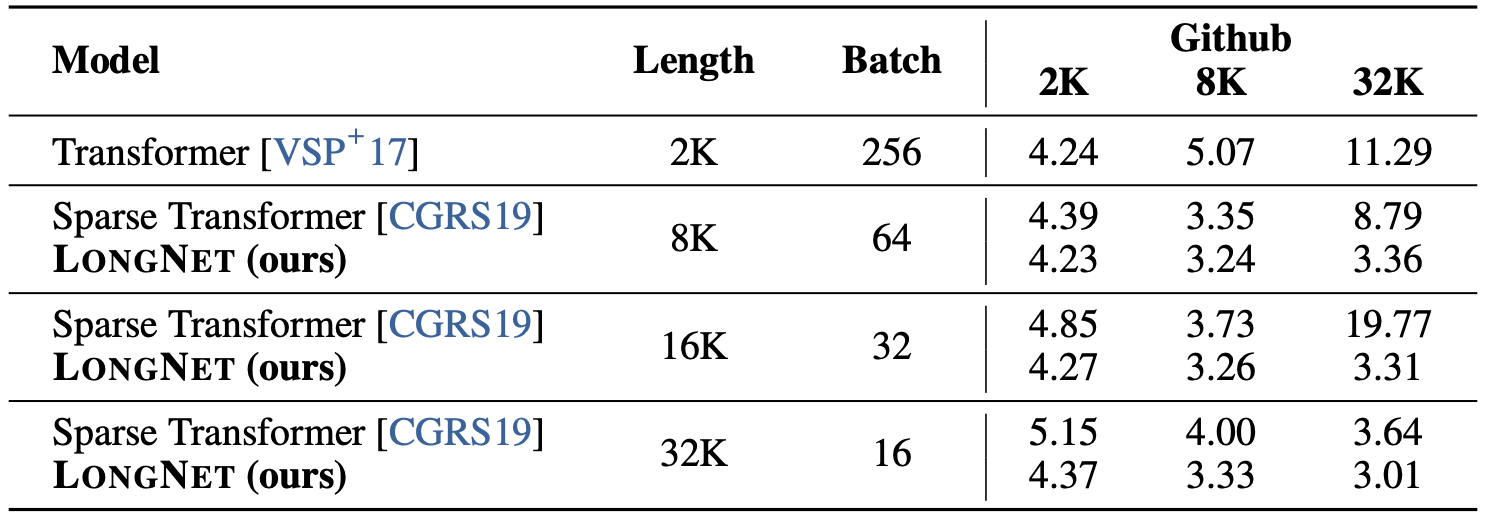
\includegraphics[width=\hsize]{longnet.png}
            \end{figure}

    \subsection{LongLoRA}
        Yukangら\cite{longlora}によって提案された、
        コンテキスト長が大きい場合でも効率的にLoRAを適用する手法。
        この手法は、Position Interpolationなどによってコンテキスト長を拡張した
        モデルに対してファインチューニングを行うことを仮定している。
        通常のLoRAではコンテキスト長が大きくなるにつれてperplexityが
        大きくなってしまう。
        一方、通常のファインチューニングは低いperplexityを維持するが、
        計算コストとVRAMの消費量が膨大になってしまう。
        LongLoRAでは、後述のShifted Sparse Attentionを用いて
        perplexityを通常のファインチューニングと同等に抑えつつ、
        VRAM消費量もLoRAと同等、
        かつより小さな計算量でのファインチューニングを実現している。

        \subsubsection{Shifted Sparse Attention}
            まず、入力シーケンスを分割し、
            分割したブロックごとにAttention機構に通す。
            これにより、計算量が改善された。
            さらに、各ブロックの大きさの半分だけずらして分割をした入力を
            同様にAttention機構に通す。
            これらのAttentionを合算することで、計算量を抑えつつ、
            ブロック間の依存関係を捉えることができる。
            Shifted Sparse Attentionの概念図を図\ref{fig:SSA}に示す。
            \begin{figure}[ht]
                \centering
                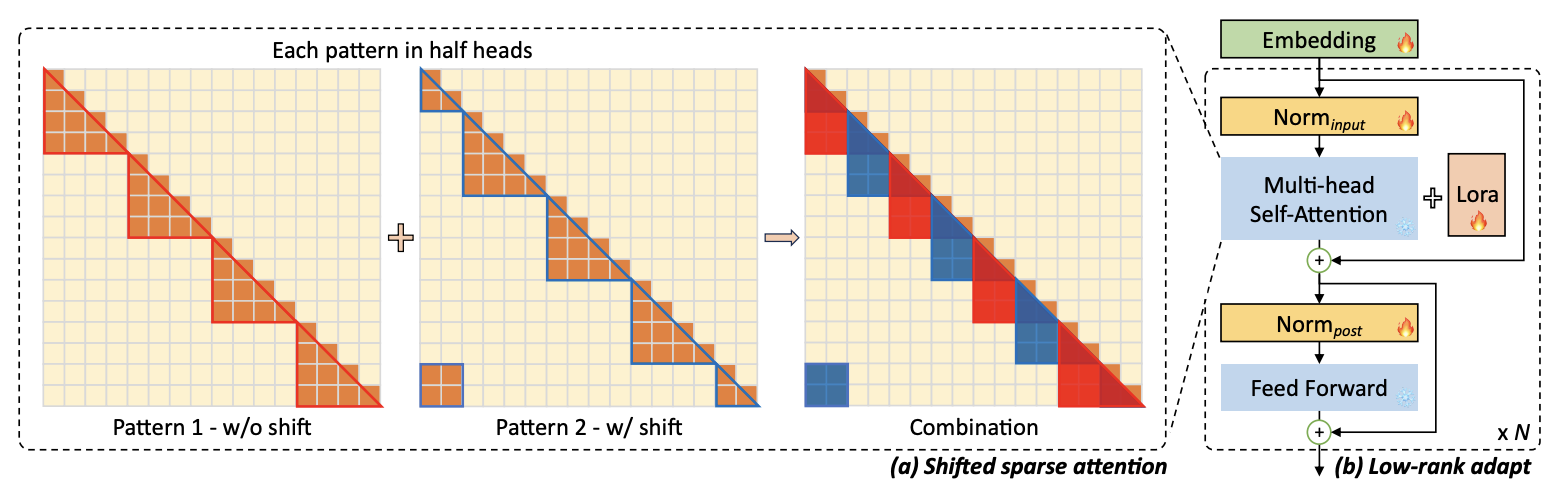
\includegraphics[width=\hsize]{ssa.png}
                \caption{Shift Sparse Attention\cite{longlora}}
                \label{fig:SSA}
            \end{figure}

        \subsubsection{実験結果}
            Perplexity、VRAM使用量、学習時間の三つの観点からLongLoRA
            の評価が行われた。
            コンテキスト長の増大に伴うそれぞれの値の変化を図\ref{fig:longlora}
            に示す。
            \begin{figure}[ht]
                \centering
                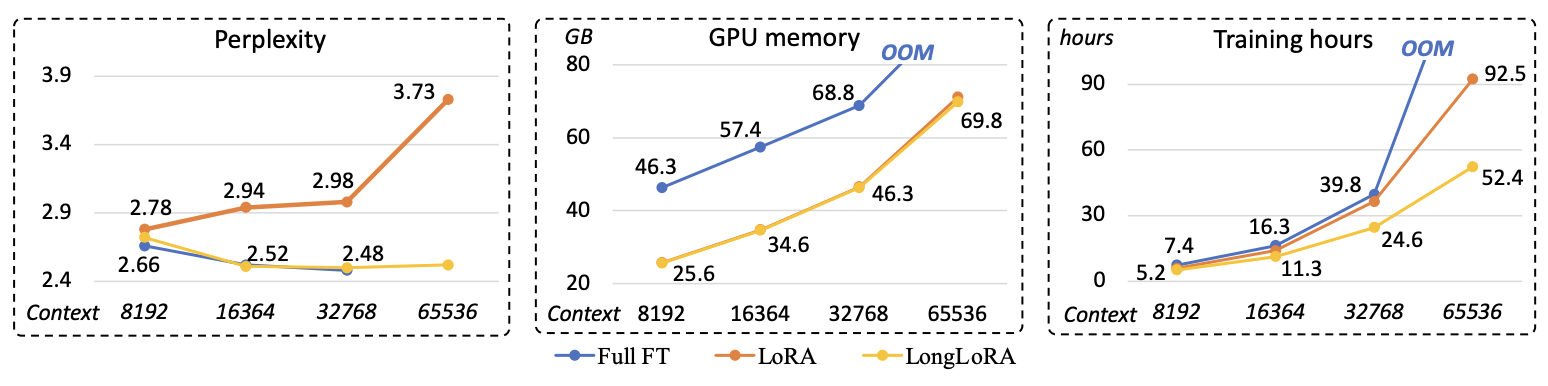
\includegraphics[width=\hsize]{longlora.png}
                \caption{LongLoRAの性能\cite{longlora}}
                \label{fig:longlora}
            \end{figure}

            図より、LongLoRAは、通常のファインチューニングと同様の性能を維持しつつ、
            LoRAと同様にVRAM使用量を抑え、
            かつLoRAより少ない時間で学習できていることがわかる。

\subsection{外挿によるシーケンス拡張}
    Yutaoら\cite{extra}は、
    transformerモデルの外挿(学習データより長いデータの入力)を可能にする手法を提案した。
    外挿能力の指標としてAttention Resolutionを定義している。
    \begin{align*}
        R(s) = \sum_{i=0}^N\frac{e^{s[i]}\left(e^{s[i]}-e^{s[i+1]}\right)}{\left(\sum_{i=0}^Ne^{s[i]}\right)^2}
    \end{align*}
    \begin{description}
        \item[$s\textrm{[}i\textrm{]}$]{
            距離が$i$の二つのトークンのAttentionスコア
            (Attention行列の要素)の期待値
        }
        \item[$R(s)$] Attention Resolution
    \end{description}

    位置エンコーディングの工夫とBlockwise Causal Attentionの二つの手法
    を用いてAttention Resolutionを最大化し、
    モデルの外挿能力を強化している。

    \subsubsection{位置エンコーディングによるAttention Resolutionの最大化}
        Attention Resolutionを増加させる為に、RoPEを改良した位置エンコーディングを提案している。
        Query,Keyそれぞれに対する以下の位置エンコーディング$f_q,f_k$を考える。
        \begin{align*}
            f_q(\q,n) = \begin{pmatrix}
                q_1\cos n\zeta^n_1\theta_1 - q_2\sin n\zeta_1^n\theta_1 \\
                q_2\cos n\zeta^n_1\theta_1 + q_1\sin n\zeta_1^n\theta_1 \\
                \vdots \\
                q_{D-1}\cos n\zeta^n_{\frac{D}{2}}\theta_{\frac{D}{2}} - q_D\sin n\zeta^n_{\frac{D}{2}}\theta_{\frac{D}{2}} \\
                q_D\cos n\zeta^n_{\frac{D}{2}}\theta_{\frac{D}{2}} + q_{D-1}\sin n\zeta^n_{\frac{D}{2}}\theta_{\frac{D}{2}}
            \end{pmatrix},f_k(\k,n) = \begin{pmatrix}
                k_1\cos n\zeta^{-n}_1\theta_1 - k_2\sin n\zeta^{-n}_1\theta_1 \\
                k_2\cos n\zeta^{-n}_1\theta_1 + k_1\sin n\zeta^{-n}_1\theta_1 \\
                \vdots \\
                k_{D-1}\cos n\zeta^{-n}_{\frac{D}{2}}\theta_{\frac{D}{2}} - k_D\sin n\zeta^{-n}_{\frac{D}{2}}\theta_{\frac{D}{2}} \\
                k_D\cos n\zeta^{-n}_{\frac{D}{2}}\theta_{\frac{D}{2}} + k_{D-1}\sin n\zeta^{-n}_{\frac{D}{2}}\theta_{\frac{D}{2}}
            \end{pmatrix}
        \end{align*}
        \begin{description}
            \item[$\q,\k$]{
                あるトークンに対するQueryとKey:
                $\q={}^t(q_1,\cdots,q_D), \k={}^t(k_1,\cdots,k_D)$
            }
            \item[$n$]{
                トークンの位置
            }
        \end{description}
        $\zeta_i$はハイパーパラメータ$\gamma$を用いて
        \begin{align*}
            \zeta_i = \frac{\frac{i}{\frac{D}{2}}+\gamma}{1+\gamma}
        \end{align*}
        で定義される定数で、$[0,1]$の範囲を取る。
        ここで、$\zeta_i=1$とすると、これはRoPEと同様の定義になる。
        この位置エンコーディングを用いた際のAttentionスコアの期待値を図\ref{fig:exp}に示す。
        図を見ると、RoPEでは発振が見られるが、
        提案手法ではそれが抑えられている。
        これにより、Attention Resolutionが増大することが確認された。
        \begin{figure}[ht]
            \centering
            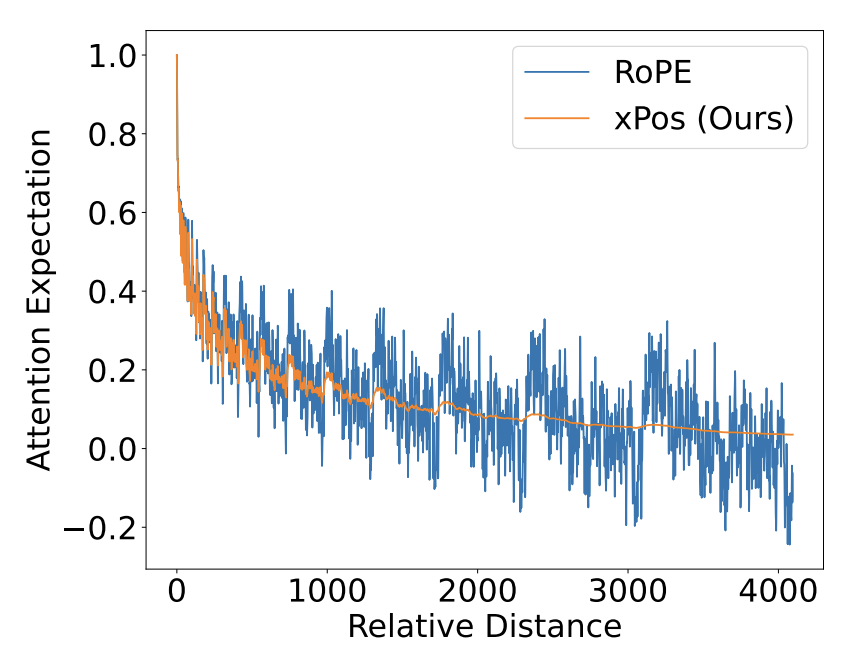
\includegraphics[width=.6\hsize]{exp.png}
            \caption{二つのトークンの相対距離に対するAttentionスコアの期待値\cite{extra}}
            \label{fig:exp}
        \end{figure}

    \subsubsection{Blockwise Causal Attention}
        出力シーケンスを入力シーケンス長の半分の長さのブロックに分割し、
        ブロックごとに順番にAttention機構に通す(図\ref{fig:block})ことで、
        間接的に離れた距離のトークン同士の情報がAttention行列に適用され、
        Attention Resolutionが増大することが示された。
        \begin{figure}[ht]
            \centering
            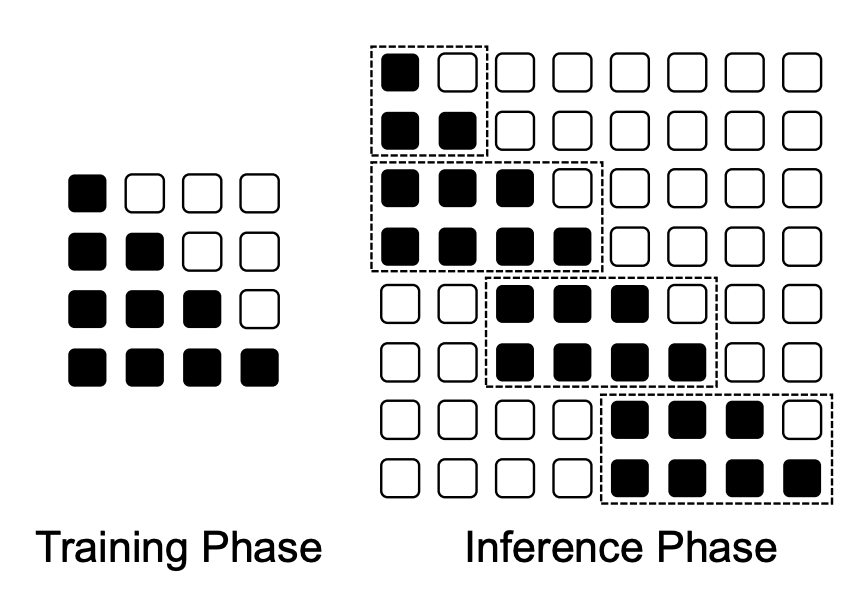
\includegraphics[width=.6\hsize]{block.png}
            \caption{
                Blockwise Causal Attention\cite{extra}
            }
            \label{fig:block}
        \end{figure}

    \subsubsection{実験結果}
        提案モデルはトークン長1024で学習し、2048トークン、
        4096トークンの入力における外挿能力が検証された。
        評価はPerplexityの比較で行われた。
        表\ref{tab:lex}に各モデルのPerplexityを示す。
        \begin{figure}[ht]
            \caption{各モデルのPerplexity\cite{extra}}
            \label{tab:lex}
            \centering
            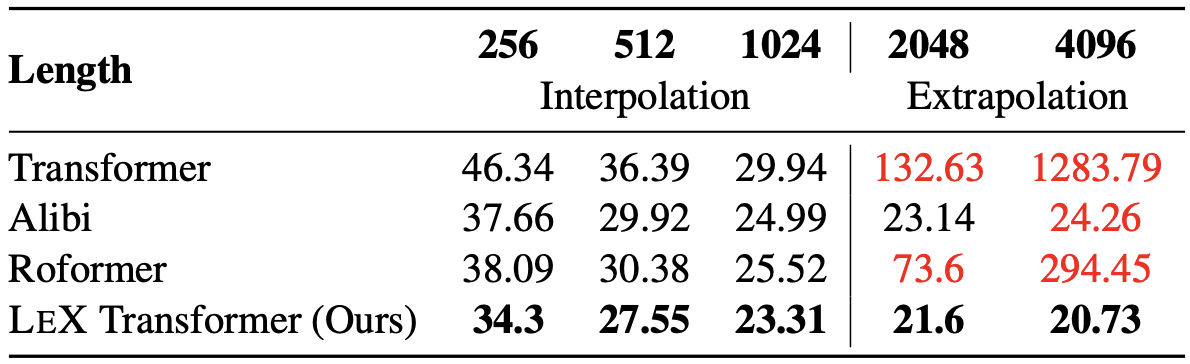
\includegraphics[width=.6\hsize]{lex.png}
        \end{figure}

        表より、提案手法は他のモデルより外挿能力に長けていることがわかった。

\section{展望}
    以上では、シーケンスの拡張を行った先行研究を見てきた。
    再学習を行う・行わない手法それぞれどちらも挙げたが、
    LLMを扱う上で、モデルの再学習は時間・空間計算量の観点で
    大きな障壁となる。
    また、理想的なLLMは入出力どちらも外挿可能なアーキテクチャであると考える。
    今後、再学習を行わずに入出力どちらも外挿可能なモデルについて調査・検証を進めていきたい。

    このような研究を行う上で、事前学習済みのパラメータを用いつつ内部構造に変更を
    加えて検証を行えるモデルが不可欠である。
    \textbf{現状、そのようなモデルが公開されているプラットフォーム等を発見できていない為、
    思い当たる方は是非平田に一報願いたい。}
    (huggingfaceにて公開されているモデル群はダメであった...)

\begin{thebibliography}{99}
    \bibitem{rope}{
        Jianlin S., et al.,
        ``RoFormer: Enhanced Transformer with Rotary Position Embedding'', \\
        arXiv:2104.09864,
        2021
    }
    \bibitem{inter}{
        Shouyuan C., et al.,
        ``Extending Context Window of Large Language Models via Positional Interpolation'',
        arXiv:2306.15595,
        2023
    }
    \bibitem{kaiokendev}{
        kaiokendev,
        ``Extending Context is Hard... but not Impossible'', \\
        `https://kaiokendev.github.io/context',
        最終閲覧日: 2024/7/8
    }
    \bibitem{yarn}{
        Bowen P., et al.
        ``YaRN: Efficient Context Window Extension of Large Language Models'',
        International Conference on Learning Representations 2024,
        2023
    }
    \bibitem{ntk}{
        bloc97,
        ``NTK-Aware Scaled RoPE allows LLaMA models to have extended (8k+) context size without any fine-tuning and minimal perplexity degradation.'', \\
        `https://www.reddit.com/r/LocalLLaMA/comments/14lz7j5/ \\ ntkaware\_scaled\_rope\_allows\_llama\_models\_to\_have',
        最終閲覧日: 2024/7/8
    }
    \bibitem{longnet}{
        Jiayu D., et al.,
        ``LongNet: Scaling Transformers to 1,000,000,000 Tokens'',
        arXiv:2307.02486,
        2023
    }
    \bibitem{longlora}{
        Yukang C., et al.,
        ``LongLoRA: Efficient Fine-tuning of Long-Context Large Language Models'',
        International Conference on Learning Representations 2024,
        2023
    }
    \bibitem{extra}{
        Yutao S., et al.,
        ``A Length-Extrapolatable Transformer'',
        Association for Computational Linguistics 2023,
        2022
    }
    \bibitem{survey}{
        Liang Z., et al.,
        ``Length Extrapolation of Transformers: A Survey from the Perspective of Positional Encoding'',
        arXiv:2312.17044,
        2024
    }
\end{thebibliography}
\end{document}